% Generated from 0514 active-maintenance evidence artifacts.
% Source data: results/ai2thor_live_gsam_wave3_4_budget6_visual_prior_v1/
%              results/ai2thor_live_gsam_mixed_challenge_budgetfix_v1/

\begin{figure}[t]
    \centering
    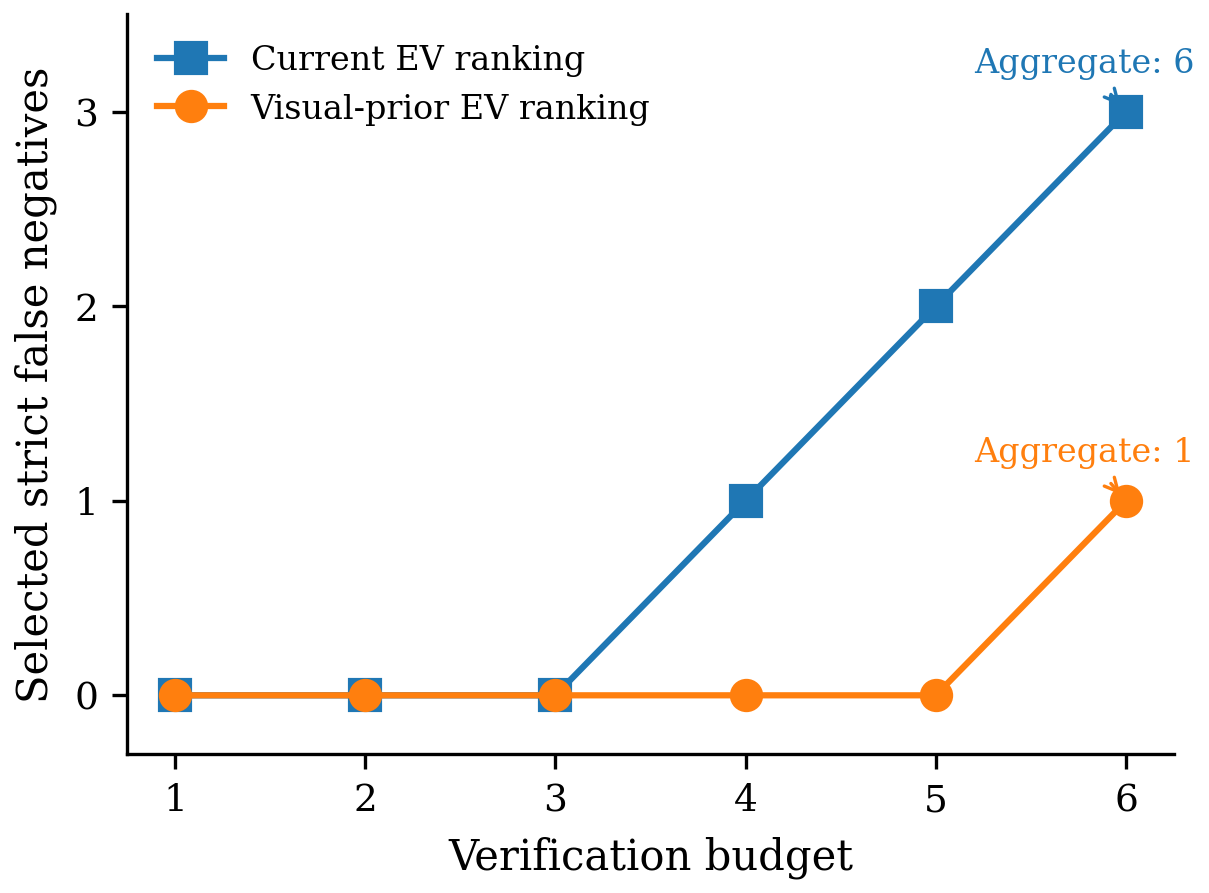
\includegraphics[width=0.48\textwidth]{figures/fig_0514_budget_curve.pdf}
    \caption{Budgeted verification curve on the targeted FloorPlan1/FloorPlan201 protocol.
    Selected strict false negatives under the current EV ranking (squares) and the calibrated visual-prior ranking (circles) over budgets 1--6.
    The visual-prior ranking reduces aggregate selected strict false negatives from 6 to 1.}
    \label{fig:budget-curve}
\end{figure}

\begin{figure}[t]
    \centering
    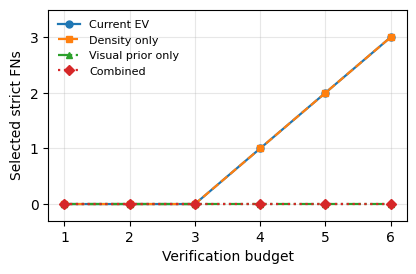
\includegraphics[width=0.48\textwidth]{figures/fig_0514_component_ablation.pdf}
    \caption{Component ablation of the expected-value signal over budgets 1--6, reported as aggregate selected strict false negatives summed over the matched counterfactual curves on the current-EV rows.
    Current and density-only each select 6; visual-only and combined each select 0.
    The hand-coded visual prior accounts for the reduction; spatial density contributes no improvement on this matched protocol.}
    \label{fig:component-ablation}
\end{figure}

\begin{figure}[t]
    \centering
    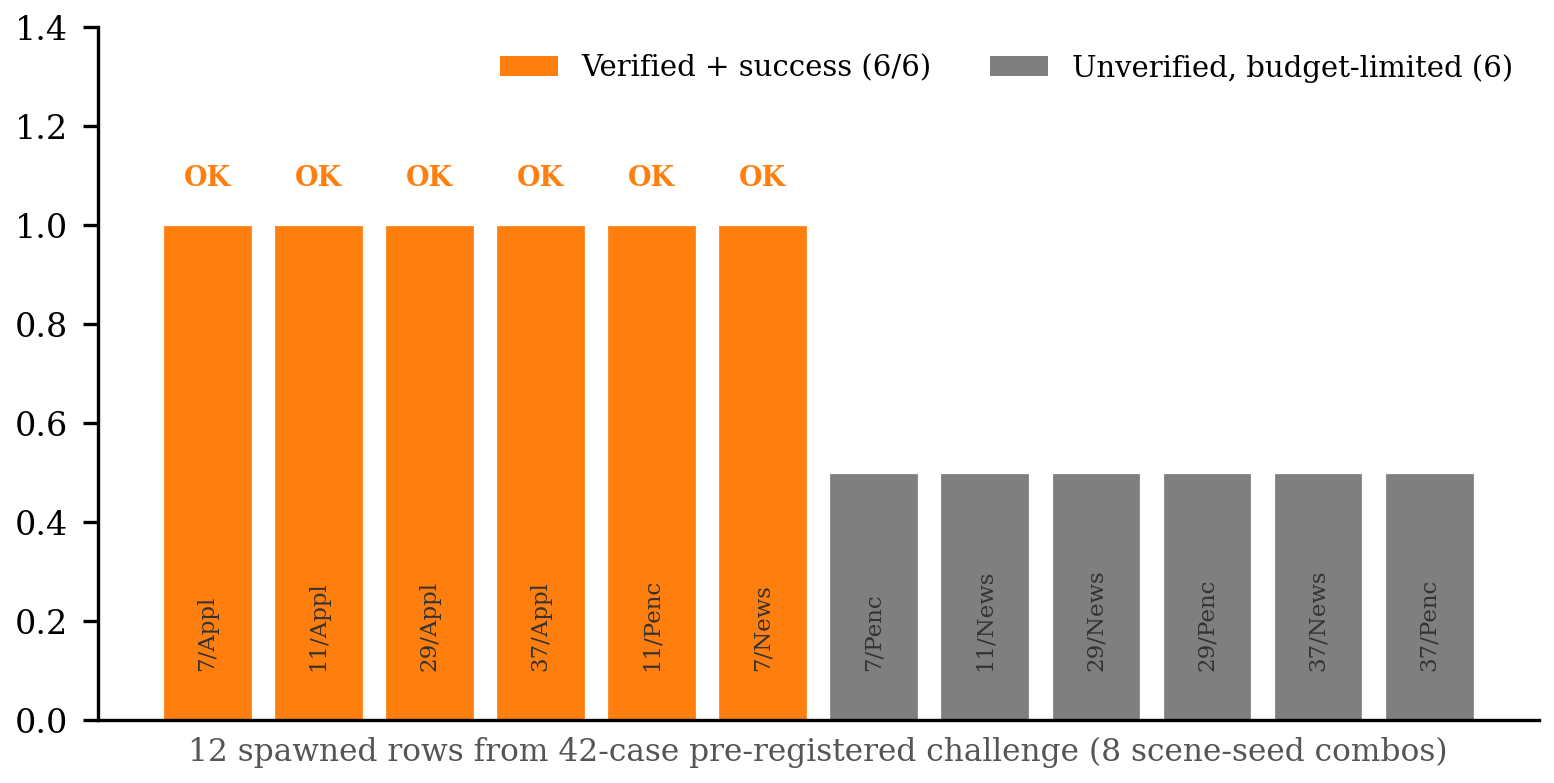
\includegraphics[width=0.95\textwidth]{figures/fig_0514_mixed_challenge.pdf}
    \caption{The fixed six-case mixed challenge: downstream PickupObject success before (grey) and after (green) adaptive stepwise action budgeting.
    The challenge moves from 2/6 to 6/6 successes without TeleportFull on measured revisit or task-bridge paths.
    This is fixed-challenge mechanism evidence, not broad scale or statistical robustness.}
    \label{fig:mixed-challenge}
\end{figure}
